\documentclass[aspectratio=169,10pt]{beamer}

\usepackage[T1]{fontenc}
\usepackage{lmodern}
\usepackage{amsmath,amssymb,booktabs,array,graphicx}
\usepackage{tikz}
\usetikzlibrary{arrows.meta,positioning,shapes.geometric}

\definecolor{navy}{HTML}{0D1F35}
\definecolor{cobalt}{HTML}{3535B8}
\definecolor{blue}{HTML}{2266AA}
\definecolor{cyan}{HTML}{34B0BF}
\definecolor{gold}{HTML}{ECB536}
\definecolor{green}{HTML}{379163}
\definecolor{red}{HTML}{C54848}
\definecolor{ink}{HTML}{232B34}
\definecolor{mid}{HTML}{637180}
\definecolor{light}{HTML}{EEF3F7}

\usetheme{default}
\usecolortheme{default}
\setbeamercolor{normal text}{fg=ink,bg=white}
\setbeamercolor{structure}{fg=blue}
\setbeamercolor{frametitle}{fg=navy,bg=white}
\setbeamercolor{title}{fg=white}
\setbeamercolor{subtitle}{fg=cyan}
\setbeamercolor{section in head/foot}{fg=white,bg=black}
\setbeamercolor{section in head/foot shaded}{fg=gray,bg=black}
\setbeamercolor{block title}{fg=white,bg=navy}
\setbeamercolor{block body}{fg=ink,bg=light}
\setbeamercolor{alertblock title}{fg=white,bg=red}
\setbeamercolor{alertblock body}{fg=ink,bg=red!8}
\setbeamerfont{frametitle}{size=\Large,series=\bfseries}
\setbeamerfont{title}{size=\LARGE,series=\bfseries}
\setbeamertemplate{navigation symbols}{}
\setbeamertemplate{itemize item}{\color{cyan}$\blacktriangleright$}
\setbeamertemplate{itemize subitem}{\color{blue}$\bullet$}
\setbeamertemplate{footline}{%
  \leavevmode\hbox{%
  \begin{beamercolorbox}[wd=.84\paperwidth,ht=2.5ex,dp=1.2ex,leftskip=.45cm]{author in head/foot}%
    \color{mid}\scriptsize Analyst Recommendations \enspace|\enspace IBES + CRSP backtest
  \end{beamercolorbox}%
  \begin{beamercolorbox}[wd=.16\paperwidth,ht=2.5ex,dp=1.2ex,rightskip=.45cm plus1fil]{date in head/foot}%
    \color{mid}\scriptsize \insertframenumber/\inserttotalframenumber
  \end{beamercolorbox}}}
\setbeamertemplate{headline}{%
  \leavevmode
  \hbox{%
    \begin{beamercolorbox}[wd=.67\paperwidth,ht=3.15ex,dp=1.25ex,leftskip=.35cm,rightskip=.25cm]{section in head/foot}
      \usebeamerfont{section in head/foot}\insertsectionnavigationhorizontal{.61\paperwidth}{}{}
    \end{beamercolorbox}%
    \begin{beamercolorbox}[wd=.33\paperwidth,ht=3.15ex,dp=1.25ex]{palette primary}
    \end{beamercolorbox}%
  }
  \vskip0pt
}
\setbeamercolor{palette primary}{fg=white,bg=cobalt}
\setbeamertemplate{frametitle}{%
  \nointerlineskip
  \begin{beamercolorbox}[wd=\paperwidth,sep=.36cm,leftskip=.1cm]{frametitle}
  \insertframetitle
  \end{beamercolorbox}
  \vspace{-0.25cm}\color{cobalt}\rule{\textwidth}{0.8pt}}

\newcommand{\smallhead}[1]{\textcolor{navy}{\textbf{#1}}}
\newcolumntype{L}[1]{>{\raggedright\arraybackslash}p{#1}}
\newcommand{\signalbox}[3]{%
  \begin{beamercolorbox}[rounded=true,sep=.55em,wd=\linewidth]{block body}
    {\color{#1}\bfseries #2}\par\smallskip #3
  \end{beamercolorbox}}

\title{Can Analyst Recommendations Predict Returns?}
\subtitle{}
\author{Chaitanya Pakala and Arsh Deep}
\date{Research design with initial IBES/CRSP cost-sensitivity results}

\begin{document}

\section{The Idea}
{\setbeamertemplate{footline}{}\setbeamertemplate{headline}{}
\begin{frame}
  \vspace{1.05cm}
  \begin{center}
  
\begin{tikzpicture}
    \node[fill=black!25,rounded corners=5pt,minimum width=13.6cm,minimum height=2.12cm,xshift=.10cm,yshift=-.10cm] {};
    \node[fill=cobalt,rounded corners=5pt,minimum width=13.6cm,minimum height=2.12cm,text width=12.6cm,align=center,text=white,font=\bfseries\LARGE] {Can Analyst Recommendations\\Predict Returns?};
  \end{tikzpicture}
  \end{center}
  \vspace{0.75cm}
  \begin{center}
    {\Large Chaitanya Pakala and Arsh Deep}
  \end{center}
\end{frame}}

\begin{frame}[shrink=10]{Why recommendations might predict returns}
\begin{columns}[T,onlytextwidth]
\column{0.48\textwidth}
\begin{block}{Research question}
Can public analyst recommendations predict \emph{subsequent} stock returns after conservative information lags and trading costs?
\end{block}
\smallhead{Economic mechanism}
\begin{itemize}\setlength\itemsep{0.35em}
  \item Analysts process firm, industry, and management information.
  \item Recommendation news may be incorporated gradually.
  \item Revisions may isolate new information better than recommendation levels.
\end{itemize}
\column{0.49\textwidth}
\begin{block}{Pre-specified hypotheses}
\begin{enumerate}\setlength\itemsep{0.35em}
  \item Favorable consensus predicts higher next-month returns.
  \item Upgrades outperform downgrades.
  \item Signals strengthen when aligned with 12--2 momentum.
  \item Effects may be larger for low-coverage firms.
\end{enumerate}
\end{block}
\begin{alertblock}{Identification target}
Return predictability must arise \textbf{after} the IBES information becomes observable---not from same-month returns, current identifiers, or missing-outcome selection.
\end{alertblock}
\end{columns}
\end{frame}

\section{Signals \& Data}
\begin{frame}[shrink=12]{Building the two signals}
\begin{columns}[T,onlytextwidth]
\column{0.43\textwidth}
\smallhead{Licensed data inputs}
\begin{itemize}\setlength\itemsep{0.32em}
  \item \textbf{IBES Summary:} ticker, CUSIP, \texttt{statpers}, \texttt{meanrec}, \texttt{numrec}.
  \item \textbf{CRSP monthly:} PERMNO, return, delisting return, price, shares, share/exchange codes.
  \item \textbf{CRSP names:} historical CUSIP intervals for point-in-time linking.
\end{itemize}
\vspace{0.15cm}
\begin{block}{Local Parquet cache}
One-time WRDS download; files are excluded from Git and reused unless \texttt{--force} is supplied.
\end{block}
\column{0.54\textwidth}
\signalbox{blue}{Consensus level}{%
\[s^{C}_{i,t}=-\,\mathrm{meanrec}_{i,t}\]
Lower IBES scores are more favorable, so the sign is reversed.}
\vspace{0.3cm}
\signalbox{cyan}{Recommendation revision}{%
\[s^{R}_{i,t}=\mathrm{meanrec}_{i,t-1}-\mathrm{meanrec}_{i,t}\]
Positive values are upgrades; negative values are downgrades.}
\vspace{0.25cm}
\smallhead{Possible extensions (not in reported results):} 12--2 CRSP momentum and analyst coverage (\texttt{numrec}).
\end{columns}
\end{frame}

\begin{frame}[shrink=3]{Making sure the timing is clean}
\centering
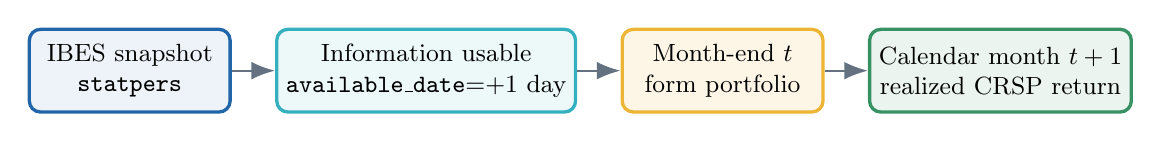
\begin{tikzpicture}[node distance=0.55cm, every node/.style={font=\small,align=center}]
\node[draw=blue,very thick,rounded corners,fill=blue!8,minimum width=2.55cm,minimum height=1.05cm] (snap) {IBES snapshot\\\texttt{statpers}};
\node[draw=cyan,very thick,rounded corners,fill=cyan!9,right=of snap,minimum width=2.55cm,minimum height=1.05cm] (avail) {Information usable\\\texttt{available\_date}=+1 day};
\node[draw=gold,very thick,rounded corners,fill=gold!12,right=of avail,minimum width=2.55cm,minimum height=1.05cm] (form) {Month-end $t$\\form portfolio};
\node[draw=green,very thick,rounded corners,fill=green!10,right=of form,minimum width=2.55cm,minimum height=1.05cm] (ret) {Calendar month $t+1$\\realized CRSP return};
\draw[-{Latex[length=3mm]},thick,mid] (snap)--(avail);
\draw[-{Latex[length=3mm]},thick,mid] (avail)--(form);
\draw[-{Latex[length=3mm]},thick,mid] (form)--(ret);
\end{tikzpicture}
\vspace{0.45cm}
\begin{columns}[T,onlytextwidth]
\column{0.49\textwidth}
\begin{block}{Availability rule}
Use the latest signal satisfying
\[
\mathrm{available\_date}_{i}\leq \mathrm{formation\_date}_{t}.
\]
A month-end snapshot cannot be traded at that same close.
\end{block}
\column{0.49\textwidth}
\begin{block}{Outcome rule}
Weights formed in month $t$ join only to calendar-month $t+1$ returns. CRSP outcomes combine
\[
(1+r_{i,t+1})(1+dlret_{i,t+1})-1.
\]
\end{block}
\end{columns}
\end{frame}

\section{Testing the Strategy}
\begin{frame}[shrink=10]{From signals to portfolios}
\begin{columns}[T,onlytextwidth]
\column{0.54\textwidth}
\begin{enumerate}\setlength\itemsep{0.42em}
  \item Keep CRSP common stocks on NYSE/AMEX/NASDAQ with price $\geq\$5$ and at least two recommendations.
  \item Rank the selected signal within each formation month.
  \item Equally weight the top decile long and bottom decile short (200\% gross exposure).
  \item Apply month-$t$ weights to month-$t+1$ total returns.
\end{enumerate}
\begin{block}{Net strategy return}
\[
r^{net}_{p,t+1}=\sum_i w_{i,t}r_{i,t+1}
-\frac{c}{10{,}000}\sum_i|w_{i,t}-w_{i,t-1}|,
\]
with baseline $c=10$ basis points.
\end{block}
\column{0.43\textwidth}
\smallhead{Strategies used for reported results}
\begin{center}\small
\begin{tabular}{@{}lll@{}}
\toprule
Signal & Weight & Holding \\
\midrule
Consensus & Equal & 1 month \\
Revision & Equal & 1 month \\
\bottomrule
\end{tabular}
\end{center}
\vspace{0.25cm}
\begin{block}{Exact implementation}
Both legs rebalance monthly and are equally weighted. Recommendations enter after a one-day lag; formation-month signals earn the following month's return. Costs are charged per dollar traded.
\end{block}
\end{columns}
\end{frame}

\begin{frame}[shrink=3]{Building a stronger version}
\begin{columns}[T,onlytextwidth]
\column{0.31\textwidth}
\smallhead{Revision $\times$ weighted basket}
\begin{itemize}\setlength\itemsep{0.38em}
  \item Start with recommendation revisions, not consensus levels.
  \item Scale positions by revision strength and reliability.
  \item Keep separate long-upgrade and short-downgrade baskets.
\end{itemize}
\column{0.31\textwidth}
\smallhead{Analyst-skill-weighted signal}
\begin{itemize}\setlength\itemsep{0.38em}
  \item Score analysts from daily IBES recommendation events.
  \item Use volatility-normalized 30-day excess returns after prior calls.
  \item Require at least 25 historical calls.
  \item Weight each new revision by the analyst's historical score.
\end{itemize}
\column{0.31\textwidth}
\smallhead{Turnover-aware construction}
\begin{itemize}\setlength\itemsep{0.38em}
  \item Feed the weighted scores into a constrained optimizer.
  \item Limit market, sector, style, liquidity, and concentration risk.
  \item Penalize turnover directly and use no-trade bands.
  \item Compare holding periods using returns after costs.
\end{itemize}
\end{columns}
\vspace{0.55cm}
\begin{block}{Design objective}
Preserve the revision signal's gross advantage while reducing the turnover that makes it unprofitable at higher trading costs. These changes are proposed next steps, not part of the reported baseline.
\end{block}
\end{frame}

\begin{frame}[shrink=9]{Guarding against false results}
\begin{columns}[T,onlytextwidth]
\column{0.49\textwidth}
\smallhead{Controls embedded in the pipeline}
\begin{itemize}\setlength\itemsep{0.30em}
  \item Historical CUSIP validity; never current-ticker matching.
  \item Signal ranking does not inspect future-return availability.
  \item Missing held outcomes invalidate the portfolio month; never set to zero.
  \item Complete entries, exits, and rebalancing count toward turnover.
  \item Duplicate PERMNO/snapshot rows fail before revision construction.
  \item Extra CRSP outcome month cannot become a new formation month.
\end{itemize}
\column{0.48\textwidth}
\smallhead{Seven automated tests currently pass}
\begin{itemize}\setlength\itemsep{0.30em}
  \item Signal unavailable before publication date.
  \item Month-end snapshot receives the one-day lag.
  \item Future revisions cannot alter past signals.
  \item Month $t$ maps to calendar month $t+1$.
  \item Delisting returns compound correctly.
  \item Missing held outcome is not treated as zero.
  \item Revision uses only the prior snapshot.
\end{itemize}
\begin{alertblock}{Real-data gate}
Before interpreting returns: audit link rate, ambiguous identifiers, duplicates, date coverage, delistings, outcome coverage, and portfolio counts.
\end{alertblock}
\end{columns}
\end{frame}

\begin{frame}[shrink=10]{Further tests worth running}
\scriptsize
\begin{tabular}{@{}L{2.65cm}L{5.45cm}L{2.55cm}L{1.55cm}@{}}
\toprule
\textbf{Extension} & \textbf{Additional design} & \textbf{Data} & \textbf{Feasibility} \\
\midrule
Momentum interaction & Double-sort revisions with trailing 12--2 returns & Existing CRSP & High \\
Coverage anomaly & Split signal efficacy by \texttt{numrec} & Existing IBES & High \\
Disagreement & Recommendation dispersion or analyst-detail cross-section & IBES optional/detail & Medium \\
Fundamentals & E/P, book-to-market, profitability, accruals & Compustat/ratios & Medium \\
Forecast revisions & Price-scaled changes in expected EPS & IBES estimates & Medium \\
PEAD interaction & Earnings surprise $\times$ recommendation revision & IBES actuals + CRSP & Medium--hard \\
Analyst skill & Condition on prior forecast/recommendation performance & IBES detail IDs & Hard \\
Broker quality & Point-in-time broker identity and classification & IBES detail + map & Hard \\
\bottomrule
\end{tabular}
\vspace{0.35cm}
\begin{alertblock}{Recommended scope}
Complete consensus and revision baselines first; then add momentum and coverage. Delay analyst/broker-level work because IBES identifiers have been reassigned historically.
\end{alertblock}
\end{frame}

\section{What We Found}
\begin{frame}[shrink=4]{Costs erase the revision advantage}
\begin{columns}[T,onlytextwidth]
\column{0.51\textwidth}
\begin{block}{Monthly baseline Sharpe by cost assumption}
\centering\large
\begin{tabular}{@{}rrr@{}}
\toprule
\textbf{Cost} & \textbf{Consensus} & \textbf{Revision} \\
\midrule
0 bps  & 0.071 & \textcolor{green}{\textbf{0.513}} \\
2 bps  & 0.059 & 0.373 \\
5 bps  & 0.041 & 0.164 \\
10 bps & 0.011 & \textcolor{red}{\textbf{$-0.186$}} \\
\bottomrule
\end{tabular}
\end{block}
\column{0.46\textwidth}
\signalbox{blue}{Consensus signal}{Sharpe is low even before costs (0.071), but it decays relatively gradually to 0.011 at 10 bps.}
\vspace{0.28cm}
\signalbox{cyan}{Revision signal}{Gross Sharpe is much stronger (0.513), yet the signal is highly cost-sensitive and becomes negative at 10 bps.}
\vspace{0.28cm}
\signalbox{gold}{Economic implication}{Any biweekly or 10-day variant must earn enough incremental signal quality to offset its likely higher turnover. Revision weighting, no-trade bands, and optimizer penalties should be tested.}
\end{columns}
\vspace{0.25cm}
\begin{alertblock}{Main conclusion}
The monthly revision strategy dominates before costs, but becomes negative at 10 bps per dollar traded. The practitioner overlays are hypotheses for improving selectivity and risk control; the current Sharpe results do not yet validate them.
\end{alertblock}
\end{frame}

\begin{frame}{Gross returns favor the revision signal}
\centering
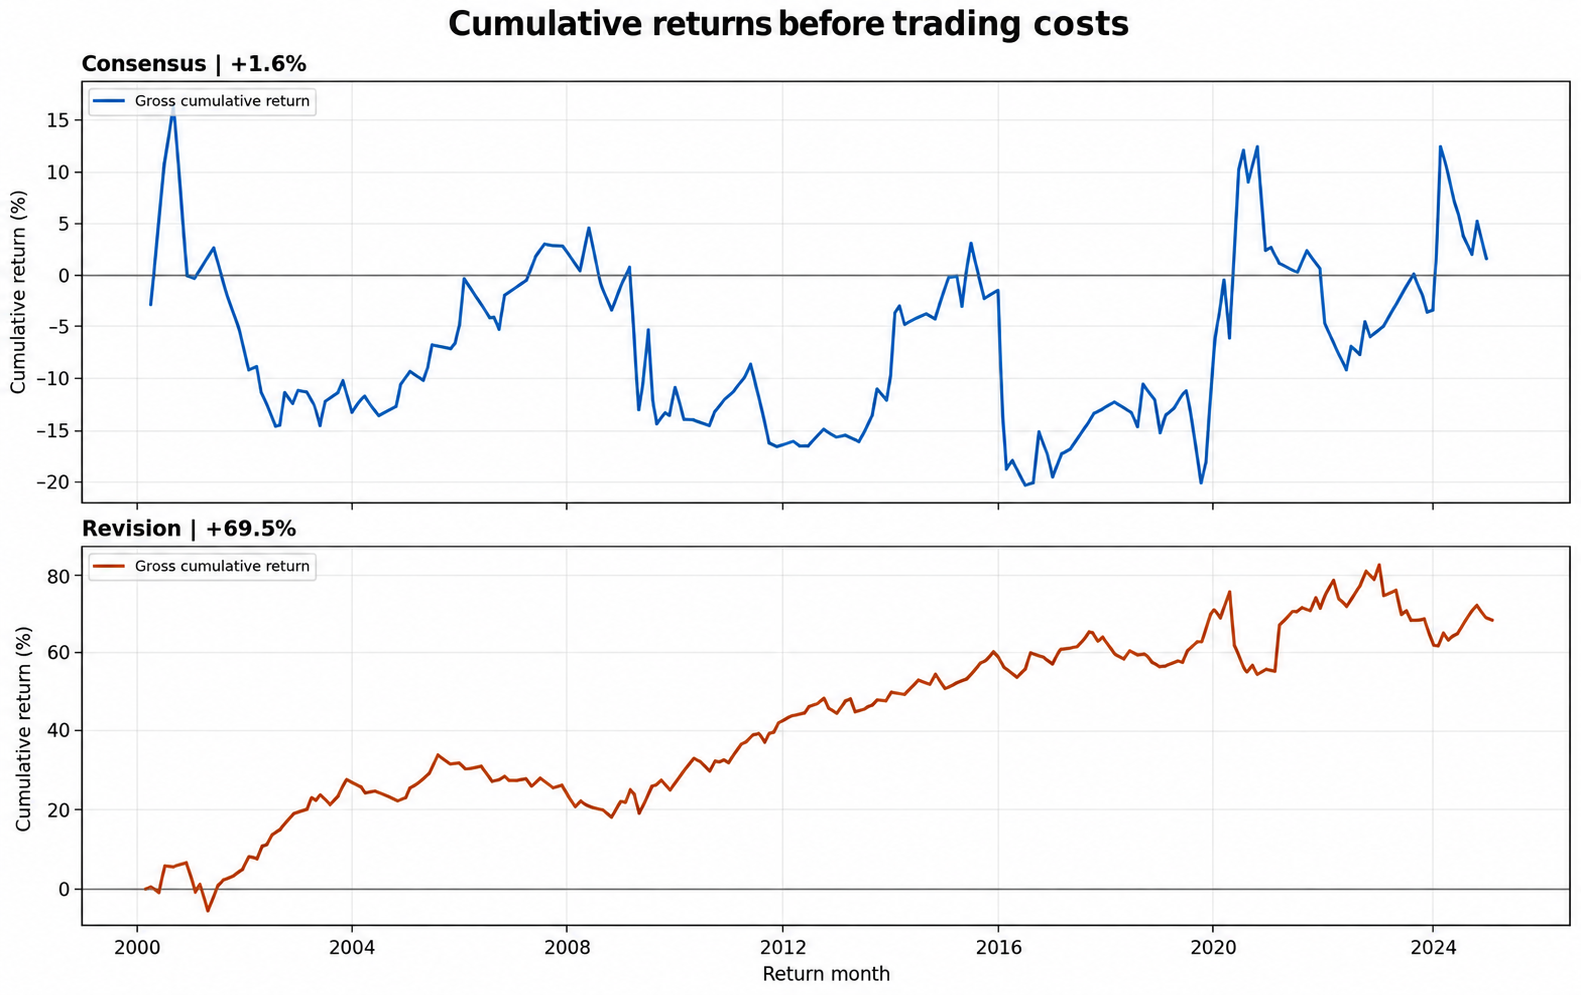
\includegraphics[width=0.93\textwidth,height=0.73\textheight,keepaspectratio]{assets/cumulative_returns_before_costs.png}
\vspace{0.08cm}

\scriptsize Gross cumulative return is approximately \textbf{+1.6\%} for consensus versus \textbf{+69.5\%} for revisions. Lines connect available months; gaps are not complete return histories.
\end{frame}

\begin{frame}[shrink=5]{Results at a glance}
\centering\small
\begin{tabular}{@{}lrrrr@{}}
\toprule
\textbf{Strategy} & \textbf{0 bps} & \textbf{2 bps} & \textbf{5 bps} & \textbf{10 bps} \\
\midrule
Consensus EW & 0.071 & 0.059 & 0.041 & 0.011 \\
Revision EW & 0.513 & 0.373 & 0.164 & $-0.186$ \\
\bottomrule
\end{tabular}
\par\scriptsize Entries are annualized Sharpe ratios under the stated per-dollar-traded cost assumption.
\vspace{0.4cm}
\begin{columns}[T,onlytextwidth]
\column{0.48\textwidth}
\begin{block}{Additional outputs to estimate}
\begin{itemize}\setlength\itemsep{0.25em}
  \item Monthly mean with HAC/Newey--West standard errors
  \item CAPM and multi-factor alpha
  \item Economic effect after transaction costs
\end{itemize}
\end{block}
\column{0.49\textwidth}
\begin{block}{Robustness}
\begin{itemize}\setlength\itemsep{0.25em}
  \item Alternative lags, holding periods, and quantiles
  \item Size, price, liquidity, and coverage screens
  \item Subperiods and equal/value weighting
\end{itemize}
\end{block}
\end{columns}
\begin{alertblock}{Interpretation rule}
Do not claim an anomaly from one favorable specification. Emphasize stability, implementation costs, factor adjustment, and the number of alternatives tested.
\end{alertblock}
\end{frame}

\begin{frame}[shrink=12]{What comes next}
\begin{columns}[T,onlytextwidth]
\column{0.48\textwidth}
\smallhead{Known limitations}
\begin{itemize}\setlength\itemsep{0.28em}
  \item WRDS schemas and entitlements differ across institutions.
  \item IBES analyst/broker identifiers have changed over time.
  \item Exact intraday publication times are generally unknown.
  \item Equal weighting can exaggerate small-stock implementability.
  \item Multiple specifications create data-mining risk.
\end{itemize}
\smallhead{Primary sources}
\begin{itemize}\setlength\itemsep{0.22em}\footnotesize
  \item WRDS I/B/E/S Overview and ICLINK documentation
  \item WRDS CRSP Monthly Stock documentation
  \item \emph{Handbook of Equity Market Anomalies}, Chapter 3
\end{itemize}
\column{0.49\textwidth}
\begin{block}{Execution plan}
\begin{enumerate}\setlength\itemsep{0.35em}
  \item Complete one-time WRDS Parquet cache.
  \item Audit schemas, links, dates, duplicates, and outcomes.
  \item Complete all metrics for the two reported EW baselines.
  \item Add factor regressions and robustness specifications.
  \item Test revision-weighted and analyst-skill variants separately.
  \item Compare monthly, biweekly, and 10-day designs after costs.
\end{enumerate}
\end{block}
\end{columns}
\end{frame}

\end{document}
